\chapter{Marco Teórico}\phantom{\cite{beetz09ijcss}}

El presente capítulo pretende dar al lector la información necesaria para entrar en el contexto de los videos digitales, los distintos tipos de segmentación que existen en ellos, así como las aplicaciones para la generación tanto de datos de validación, como de información semántica en ellos. Se menciona las características principales de dichas herramientas, sus pros y contras, y se provee algunas capturas de pantalla para que se aprecie las interfaces de usuario. Además se presenta en el capítulo las diversas bibliotecas y \textit{frameworks} de software libre que se encuentran disponibles para la elaboración de aplicaciones web. Finalmente se presenta los dos modelos más comunes de bases de datos que se utilizan para el desarrollo web y el patrón de diseño MVC.

\section{Videos digitales}

Para comprender de videos digitales es necesario primero tener los conceptos claros de los componentes en una imagen digital. Una imagen se puede definir como una función de dos dimensiones $f(x,y)$ en donde $x$ y $y$ son coordenadas espaciales en un plano y la amplitud de $f$ en cualquier par ordenado $(x,y)$ es la intensidad en escala de grises en dicho punto. Cuando $x$, $y$, y la amplitud $f$ son valores finitos y discretos, se dice que la imagen es digital. Por esta razón, toda imagen digital está compuesta por un número finito de elementos, los cuales tienen una posición particular y un valor de intensidad específico. A estos elementos se les llama pixeles. [\cite{digitalImage}]\\

Cuando las imágenes son a color, en lugar de estar en una escala de grises, existen diferentes formas de representar los colores. A estas representaciones se les llama modelos de espacio de color. Entre los más comunes se encuentran:

\begin{itemize}

	\item \emph{RGB}, se basa en la suma de los tres colores primarios (rojo, verde y azul) percibidos por el ojo humano para representar las diferentes longitudes de onda visibles del espectro electromagnético. Este modelo es utilizado por la mayoría de dispositivos electrónicos que funcionan como monitores o pantallas.
	
	\item \emph{CMY o CMYK}, se basa en la substraer de un fondo blanco los colores cyan, magenta, y amarillo para representar los demás colores. La única diferencia entre CMY y CMYK es que uno incluye el negro (K) como parte del modelo. Este modelo es utilizado por dispositivos como impresoras ya que al imprimir en papel, se empieza sobre un medio que ya es blanco y es más eficiente sustraer que agregar para formar los colores.
	
	\item \emph{HSI o HSB}, es el modelo que se basa en matiz, saturación e intensidad. El matiz se selecciona a partir de un ángulo, en el cual se varía en el espectro electromagnético visible, la saturación es ``cuanto'' de ese matiz está presente, y la intensidad o brillo dice que tan claro o intenso se ve el color. La Figura \ref{fig:hsb} muestra una cono que ayuda a visualizar la descripción.	
	
\end{itemize}

\begin{figure}
	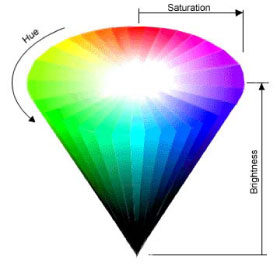
\includegraphics[width=0.4\linewidth]{images/hsb}
	\caption{Espacio de color HSI} \label{fig:hsb}
\end{figure}

Finalmente, si cada imagen en escala de grises puede ser representada como una matriz de $M \times N$ pixeles en la que cada posición $(i,j)$ tiene la intensidad del gris, una imagen en RGB se descompone en tres matrices independientes. La matriz R tiene la intensidad del rojo, la matriz G tiene la intensidad del verde y la matriz B tiene la intensidad del azul. Al sobreponer cada una de estas matrices en una sola, es cuando el ojo humano percibe un color específico.

Con todo esto en mente, ya se tiene una idea general de la representación de una imagen digital a color. Ahora bien, un video digital no es más que la reproducción de diferentes imágenes digitales a una tasa definida. A esta tasa se le denomina FPS, del inglés \emph{frames per second} que significa cuadros (imágenes) por segundo.

En términos matemáticos, un video en escala de grises puede ser representado como una función discreta de intensidad $I = f(x,y,t)$ en donde $x$ y $y$ son las coordenadas cartesianas de los pixeles que componen la imagen y $t$ es el número de cuadro actual. Cuando se reproduce el video se visualiza la matriz de intensidades de $M \times N$, y se aprecia como esta varía dependiendo del valor actual de $t$, el cual en una reproducción normal siempre varía de la forma $t = t+1$. Como se aprecia en la a Figura \ref{fig:frames}, en una línea del tiempo de un segundo, los cuadros van pasando de manera que solo uno de ellos se visualiza a la vez y crea la sensación de estar viendo un movimiento continúo. 

De manera análoga a la imagen RGB, un video en el espacio de color RGB es representado por tres funciones de intensidad, cada una asignada a los colores rojo, verde y azul respectivamente. De esta manera el video a color resulta de sobreponer las matrices que tienen en sus entradas $(i,j)$ el resultado de las funciones $R = r(x,y,t)$, $G = g(x,y,t)$ y $B = b(x,y,t)$ con $x=i$, $y = j$ y $t$ el número de cuadro actual.

\begin{figure}
	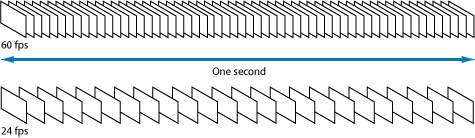
\includegraphics[width=\linewidth]{images/frames}
	\caption{Descripción gráfica de la cantidad de cuadros en un segundo} \label{fig:frames}
\end{figure}

La Figura \ref{fig:frames} muestra además de manera gráfica como dependiendo de la tasa de FPS, en un solo segundo se tiene un número diferente de cuadros. Sigue siendo un debate científico el saber el máximo de cuantos cuadros es capaz de detectar el sistema visual del cuerpo humano. Sin embargo, es sabido que se puede procesar entre 10 a 12 cuadros por segundo y que estos sean identificados como imágenes independientes y no como una secuencia perteneciente a un video. Debido a esto, existió la tendencia a pensar que si se duplicaba dicha cantidad, las personas no percibirían diferencia alguna, por ello alrededor de los 1920's las películas del cine mudo tenían tasas entre los 20 y 24 FPS.

Desde ese entonces, los 24 cuadros por segundo se convirtieron en un pseudo-estándar para películas y transmisiones de televisión. La razón es sencilla, la relación de costo y calidad llega a estar en un punto de equilibrio. No tenía sentido en su momento grabar, y reproducir a más cuadros porque se requería más almacenamiento y más capacidad de procesamiento y al final la diferencia no sería lo suficientemente notoria. Ahora hay tres estándares que son 24p, 25p y 30p; sin embargo, tener diferentes tasas de FPS tiene diversas aplicaciones.

En el mundo artístico grabar a más cuadros por segundo luego tiene la posibilidad de reproducir secuencias en cámara lenta, y grabar a menos cuadros por segundo, tiene la utilidad de crear lo que se conoce como \emph{time-lapse}, que es una secuencia rápida de imágenes que en realidad representan lo que sucedió en una gran cantidad de tiempo. También se está experimentando en el cine ahora grabar a 48p para aumentar un poco el sentido de realidad.

En aplicaciones científicas, obtener una tasa más alta de cuadros por segundos puede aumentar la precisión de las mediciones. Existen cámaras infrarrojas que graban hasta a 300 FPS, que pueden captar movimientos con precisión milimétrica. En el procesamiento digital de videos y en el reconocimiento de patrones, por lo general los algoritmos procesan los videos cuadro por cuadro, ya que esto da mejores resultados a la hora de obtener datos y realizar mediciones. Cada cuadro es una imagen independiente, por lo que la información en ella varía y para poder identificar si un algoritmo de procesamiento funciona correctamente se tiene que revisar cuadro a cuadro la información que provee el algoritmo y la que percibe una persona, por esta razón los datos de validación deben de ser generados de la misma manera. 

No toda la información contenida en un video digital es de interés para un objeto de estudio específico. Por dicha razón existen diversos tipos de segmentación que son realizados para ordenar el video de cierta manera en la cual se puedan obtener datos, mediciones e información de una manera correcta. Dichas formas de segmentar los videos son explicadas en la siguiente sección.

\section{Tipos de segmentación en videos}

En general, en toda aplicación de reconocimiento de patrones debe de llevarse a cabo la segmentación, la cual consiste en dividir o segmentar una fuente de información en diferentes partes y de diversas maneras con el fin de obtener un elemento que provea mayor información o que sea más fácil de analizar.

Para el caso de las imágenes digitales puede segmentarse de tal manera que cada uno de sus pixeles pertenezca a un conjunto que comparta ciertas características con otros pixeles y se les asigna una misma etiqueta. En la Figura \ref{fig:imgseg1}, tomada de la publicación \textit{Contour Detection and Hierarchical Image Segmentation} \cite{imgseg}, se puede apreciar como la segmentación de la imagen se realizó para encontrar los pixeles que pertenecen a los bordes, y así poder visualizar de manera más clara cuales son los contornos de las dos aves. 

\begin{figure}
	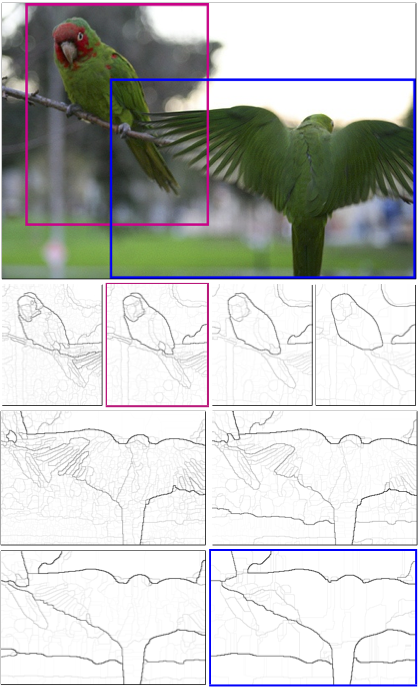
\includegraphics[width=0.63\linewidth]{images/imgseg}
	\caption{Segmentación de imágenes para obtener los contornos.} \label{fig:imgseg1}
\end{figure}

De igual manera, los videos digitales también se segmentan para facilitar su análisis y llegar a obtener información de los mismos. La tesis doctoral \emph{Automated Semantic Annotation of Football Games from TV Broadcast} realizada por Francisco \cite{siles1} describe el procedimiento seguido para poder crear un sistema automatizado para la anotación semántica de partidos de fútbol a partir de transmisiones de televisión. Este es un excelente caso para especificar los diferentes tipos de segmentación que puede ser necesario realizar en videos para llegar a obtener contenido realmente relevante de ellos. Se toma como ejemplo el caso de los partidos de fútbol de las tesis doctoral previamente mencionada para realizar la explicación de los diferentes tipos de segmentación que son te interés en este proyecto. El primero es la segmentación temporal y se describe a continuación.

\subsection{Segmentación Temporal}

Como se describió anteriormente, los videos pueden representarse como una función $f(x,y,t)$ de intensidad de grises (o $r(x,y,t)$, $g(x,y,t)$, $b(x,y,t)$, intensidades para cada uno de los colores en el espacio RGB), en la cual las posiciones $x$ y $y$ son las respectivas al pixel en cuestión y $t$ es una posición en la línea del tiempo. Debido a esta característica cambiante en el tiempo, el primer tipo de segmentación en videos es la temporal. En este se segmenta a nivel de escenas, identificando cuales de ellas son útiles para el tipo de información que se desea extraer del video y cuales no. 

Para realizar la segmentación temporal, primero se deben encontrar las transiciones del video. Se ubica el número de cuadro $t$ en el cual inicia una transición de escena, y un número de cuadro $t+n$, donde $n$ es el número de cuadros que dura la transición. Cuando esta acaba se llega a un tipo de escena que puede o no ser relevante para el análisis. Se sabe que todos los cuadros que pertenezcan a una transición, no son útiles para obtener información. Lo que se debe analizar son los cuadros entre el final de una transición y el inicio de la siguiente. Estas escenas componen la segmentación temporal de los videos.

En la transmisión de partidos de fútbol, por ejemplo, se utiliza efectos de edición, se realiza tomas del público, de las afueras del estadio, entre otros; con el fin de darle una experiencia más completa y entretenida a los espectadores de la transmisión. Sin embargo muchas de esas escenas no son de utilidad debido a que no acercan al investigador al objetivo final. Por esta razón el primer paso es identificar las escenas que si sean relevantes debido a que proveen el tipo de información que es necesaria. 

En el caso de la tesis doctoral de \cite{siles1} las escenas que son relevantes para realizar la toma de datos son las que fueron realizadas desde largo, y son descritas como \emph{far-views}. Por esta razón el primero paso fue detectar cortes, efectos, y los tipos de tomas que son irrelevantes para el objetivo final.

Al finalizar la segmentación temporal, se puede pasar a identificar en las escenas de interés los objetos que agregan valor, y ese es el siguiente tipo de segmentación. 

\subsection{Segmentación Espacial}

Continuando el ejemplo de los partidos de fútbol, una vez identificadas las escenas del tipo \emph{far-view}, se procede a hallar y ubicar espacialmente los jugadores presentes en cada toma. A este proceso se le conoce como segmentación espacial y tiene tres componentes principales los cuales son:

\begin{itemize}
	\item El \emph{\textbf{contorno}} identifica los pixeles que forman parte de los bordes o límites físicos de un objeto específico.
	\item La \emph{\textbf{posición}} por lo general es el promedio geométrico de los puntos que forman parte del contorno.
	\item La \emph{\textbf{trayectoria}} es el movimiento que describe el objeto en el tiempo, es decir, como varía la posición de un objetivo específico en cada cuadro del video.
\end{itemize}

Finalmente con dichos datos, se puede proceder a darles un sentido lógico, con lo que se tiene el último tipo de segmentación que se expone en la siguiente subsección.

\subsection{Segmentación Semántica}

Una vez que se tiene los datos de donde están los jugadores y como se mueven en el tiempo, y estableciendo relaciones entre cuales son los de un equipo u otro, se puede dar valor semántico a los datos. Por ejemplo se puede identificar cuando un equipo defiende si los jugadores se comprimen en el borde del área de penal y si el otro equipo tiene más posesión de la bola. También se podría identificar un contraatque si un equipo vuelve con gran rapidez a su propio campo y el otro se desplaza hacía el marco contrario con varios jugadores que suben a gran velocidad con posesión del balón. A esta información significativa acerca de los eventos de un video, se le conoce como segmentación semántica.



Siguiendo estos tipos genéricos de segmentación en videos, es posible obtener el contenido semántico que es el que provee la información relevante.

\subsection{Otro ejemplo de segmentación en videos: análisis de muestras de células}

De la misma manera en que se realizó la segmentación en los videos de fútbol para simplificar su análisis y llegar a obtener información semántica de los mismos, se puede realizar el mismo procedimiento para otro tipo de videos. Por ejemplo un video de una muestra de células.


En otros casos, como el análisis de eventos a nivel celular, la mitosis por ejemplo, no es relevante todo el tiempo en que se calibra el microscopio, o cuando los tintes no han hecho el efecto necesario para exponer los elementos de manera correcta. Todos estos segmentos pueden ser identificados e ignorados puesto que no hacen diferencia alguna en el estudio.

En el ejemplo del análisis de la mitosis, la segmentación espacial vendría a ser ubicar cada uno de los elementos que componen la célula: núcleo, aparato de Golgi, retículo endoplasmático, lisosomas, ribosomas, mitocondrias, membrana, entre otros y guardar los datos de sus contornos para poder ubicar su posición, y trayectorias.


En el caso de la célula, el analizar como se posicionan y mueven los los elementos dentro de ella, la alineación de los cromosomas, hasta la deformación y división de la membrana; puede proveer la información necesaria para identificar que en ese instante se dio el proceso de mitosis.

\section{Herramientas existentes para generar datos de validación para los diferentes tipos de segmentación}

En esta sección se presenta cuatro herramientas que pueden ser utilizadas para generar datos de validación: Sensarea, ViperGT, Vatic y VideoANT. Se expone la GUI de cada una, así como los tipos de segmentación que logran cubrir y algunas de sus ventajas y desventajas.

\subsection{Sensarea}

Sensarea es la herramienta más completa que se encontró para la generación de los datos de segmentación espacial. Es un software para sistemas operativos de Windows. Este se presenta como un editor que permite agregar diversas mascaras de manera manual o semiautomática al contenido espacial de un video digital. Según su creador Pascal Bertolino, la herramienta no fue diseñada con la meta de ser utilizada para la generación de datos de validación, sino como un editor inteligente que permite agregar efectos con selecciones semiautomáticas, y poder añadir información a los elementos del video. Sin embargo, aunque no sea su meta inicial, la aplicación puede ser utilizada a niveles básicos para la generación de datos manuales de validación de segmentaciones espaciales y semánticas, ya que permite exportar las coordenadas de las máscaras generadas manualmente en un archivo XML, y las etiquetas asignadas a las mismas. Si al lector le interesa ahondar más en las funcionalidad de Sensarea como editor de videos y no como generador de datos de validación, puede encontrar en las referencias la publicación: ``Sensarea: an Authoring Tool to Create Accurate Clickable Videos'' [\cite{bertolino}].

En cuanto a los inconvenientes que presenta la herramienta, se encuentra la precisión a la hora de generar los datos. Si se genera las máscaras con la herramienta de ``Brush'' del Sensarea la precisión era un poco aleatoria. No se toma en cuenta todos los pixeles que conforman el contorno, sino algo muy similar a las aristas del polígono convexo que incluye los puntos extremos (\textit{Convex Hull} de un set de puntos), por lo que no es útil para comparar con lo algoritmos que incluyen todos estos puntos y no se desea realizar una interpolación a este nivel porque sería una pérdida grande de exactitud. Para solventar dicho inconveniente, se puede utilizar la herramienta ``Vectorize Mask'' de Sensarea, pero esta es sumamente lenta, ya que para agregar un pixel, hay que darle click al mismo, así la precisión depende directamente de la cantidad de clicks utilizados para la realización del contorno, lo que termina haciendo la tarea aún más tediosa de lo que ya era.

La Figura \ref{fig:sensareaP} muestra lo descrito en el párrafo anterior de manera visual. Los puntos que se despliegan en los contornos de ambas imágenes son los que al final son exportados en el XML, por lo tanto, serían los datos que se utilizarían para realizar la validación. Los puntos de la figura \ref{fig:sens1} son muy pocos, y los de la figura \ref{fig:sens2} pueden ser suficientes para no tener mucha pérdida de precisión en la verificación del algoritmo, pero el generarlo significa dar un click por cada punto, lo cual no es eficiente.

Sensarea provee una GUI intuitiva, pero con más funcionalidades que no son relativas a la generación de datos como se puede apreciar en la Figura \ref{fig:sensareaGUI}. Por lo que se ocupa un poco de tiempo para aprender a utilizar las herramientas disponibles que si son útiles para esto. Además no cuenta con alguna forma sencilla para la generación de datos para el caso de trayectorias ni para la segmentación temporal. Finalmente a la hora de cargar videos, si estos pesan más de 100 MB, la carga suele ser lenta, con videos que son de GBs de tamaño, se puede tardar hasta 15 minutos cargando y se suele cerrar el programa de manera inesperada por algún tipo de error.

\begin{figure}
	\centering
	\begin{subfigure}[b]{0.3\textwidth}
		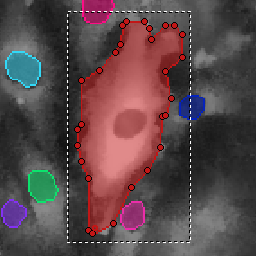
\includegraphics[width=\textwidth]{images/sens1}
		\caption{Contorno generado con la herramienta de brocha de Sensarea}
		\label{fig:sens1}
	\end{subfigure}\qquad%
	~ %add desired spacing between images, e. g. ~, \quad, \qquad, \hfill etc.
	%(or a blank line to force the subfigure onto a new line)
	\begin{subfigure}[b]{0.3\textwidth}
		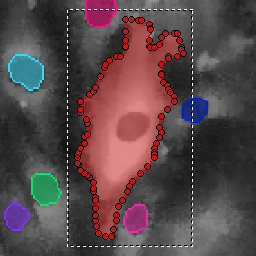
\includegraphics[width=\textwidth]{images/sens2}
		\caption{Contorno generado con la herramienta de vectores de Sensarea}
		\label{fig:sens2}
	\end{subfigure}
	\caption{Problemas de precisión encontrados en Sensarea}\label{fig:sensareaP}
\end{figure}

\begin{figure}
	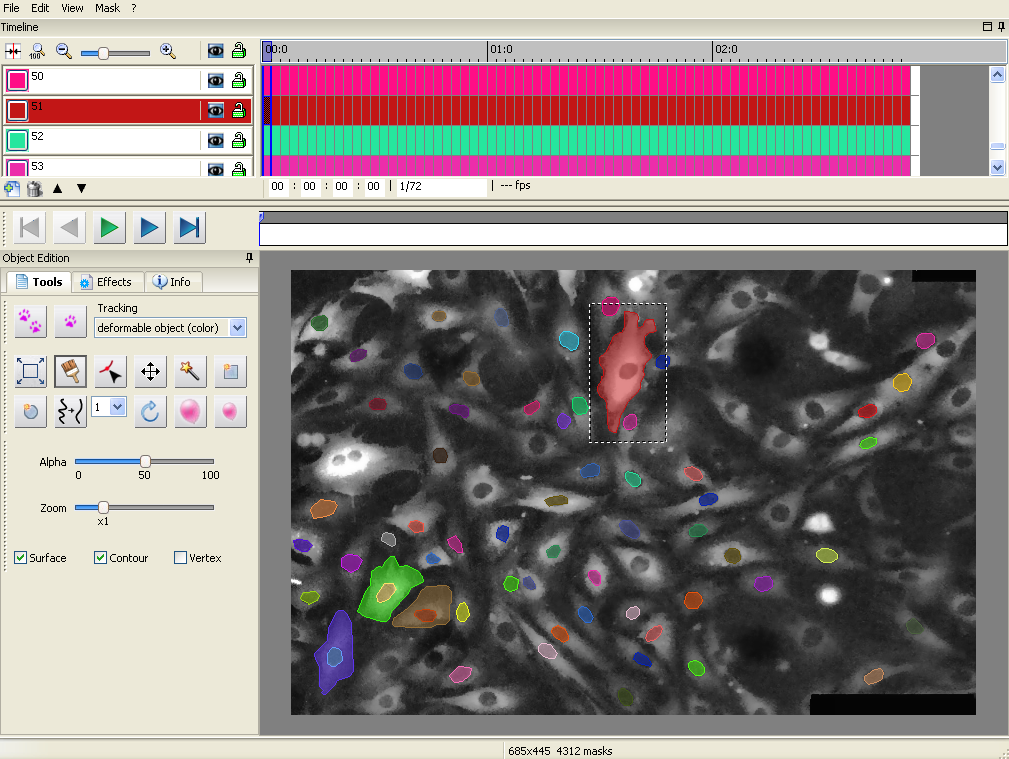
\includegraphics[width=1\linewidth]{images/sens3}
	\caption{GUI de Sensarea.} \label{fig:sensareaGUI}
\end{figure}


\begin{figure}
	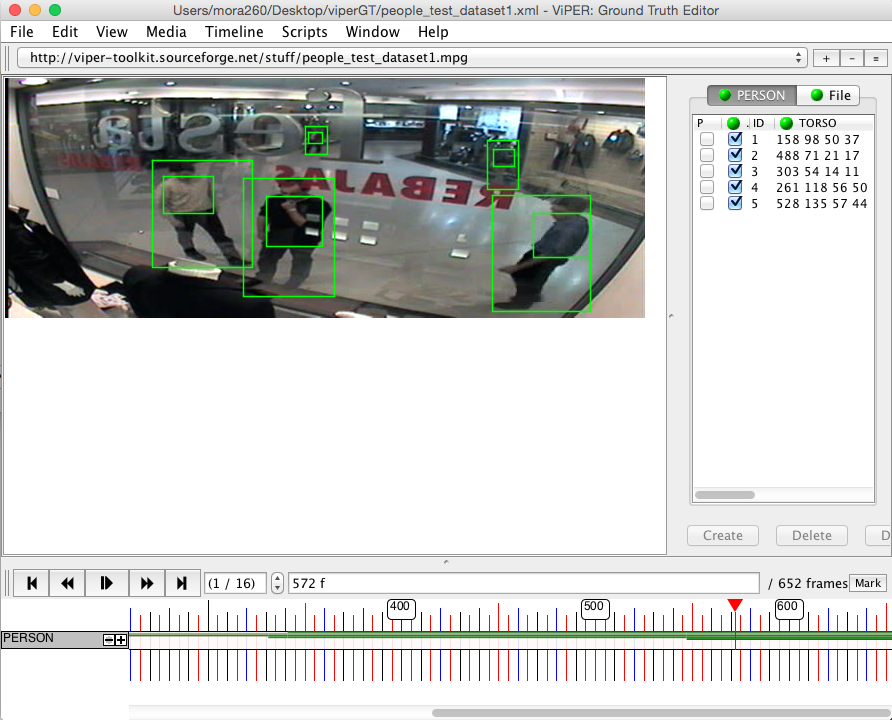
\includegraphics[width=0.95\linewidth]{images/viper}
	\caption{GUI de ViperGT.} \label{fig:viperGUI}
\end{figure}


\subsection{ViPER-GT}

ViPER-GT fue una de las primeras herramientas para la anotación de videos y generación de datos de validación. Fue creada por el laboratorio LAMP, del inglés \emph{Language And Media Processing Laboratory}, y pertenece al conjunto de herramienta ViPER que son \emph{The Video Performance Evaluation Resource}. Además entre las funcionalidades que provee está identificar objetos con cuadros y agregar una etiqueta sobre el tipo de objeto como lo muestra la Figura \ref{fig:viperGUI} y es multiplataforma debido a que su ejecutable es un .jar de Java. Dicho esto, se puede concluir que el único tipo de segmentación que se puede validar adecuadamente es la espacial, excluyendo los contornos.

Entre las mayores limitaciones está que solo permite cargar correctamente videos en un contenedor de tipo mpg, y en codecs muy desactualizados. Además la interfaz no es intuitiva y empezar a realizar anotaciones puede tornarse complicado. Para comprender como se utiliza la herramienta, lo mejor es cargar uno de los proyectos de ejemplo que están en la página de documentación, ya que de esta manera las ventanas de la interfaz gráfica cargan sus contenidos y ya se puede saber para que funcionan. Debido a que no se pueden cargar videos en formatos más utilizados y que la interfaz no era intuitiva y no se permitía realizar contornos no se continuó utilizando la herramienta y se prefirió continuar la investigación con otras.

\subsection{VATIC}

\begin{figure}
	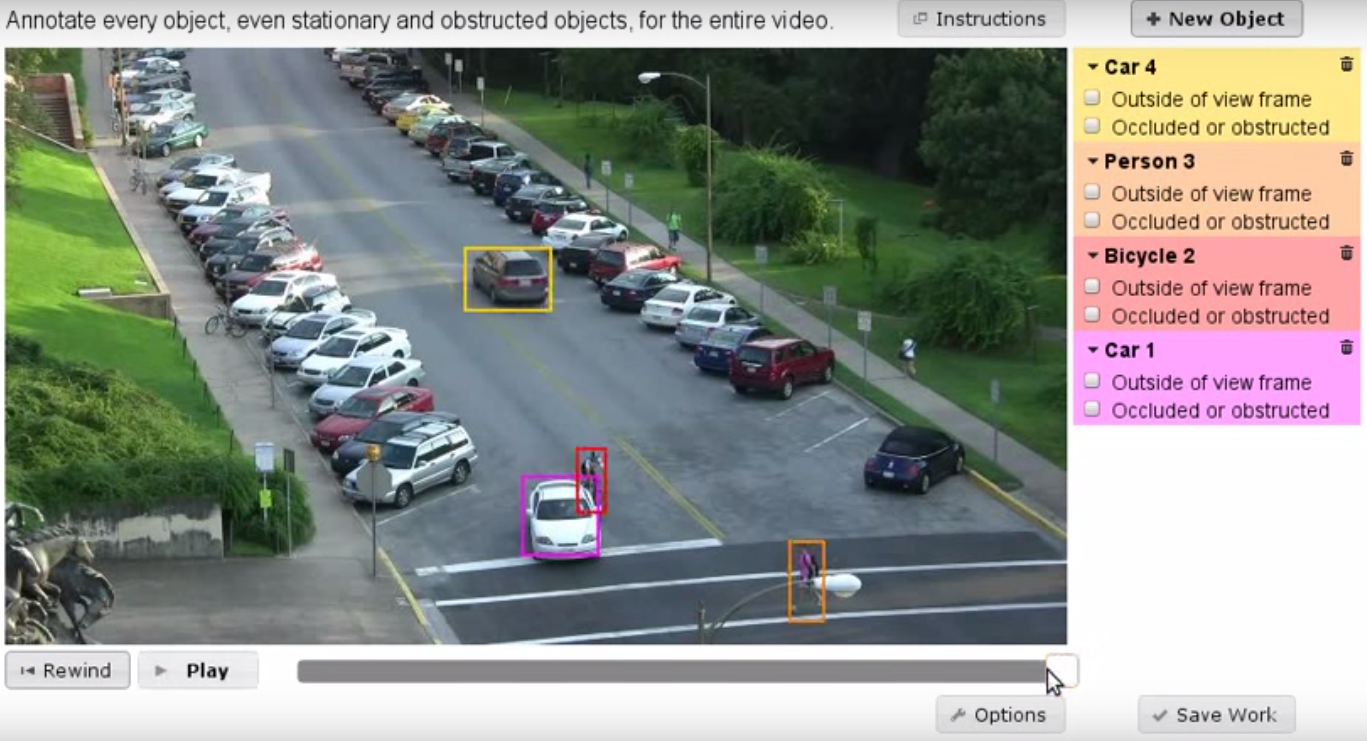
\includegraphics[width=1\linewidth]{images/vatic}
	\caption{GUI de VATIC.} \label{fig:vaticGUI}
\end{figure}

Video Annotation Tool from Irvine, California o por su acrónimo, VATIC, es una herramienta en línea para la anotación de videos para ayudar a la investigación de visión por computador. El hecho de que sea web no significa que actualmente este en un servidor con todas sus funcionalidades disponibles como un servicio abierto, sino que cuando se instala y configura, uno lo puede poner a funcionar como un servicio web, ya que está hecho para correr en un servidor Apache. Según la documentación, el sistema solo ha sido probado en Ubuntu con un servidor Apache 2.2 y una base de datos a través de un servidor MySQL.

Dicho esto, se tiene el primer problema de la herramienta, no es fácil de instalar. Se requiere tener experiencia con servidores y utilización de diversas bibliotecas para poder poner a funcionar el programa por primera vez. No se proporciona un script que automatice la instalación ni si quiera en el sistema operativo en el cual esta probado. Además la mayoría de funcionalidades como cargar videos, realizar cortes de cuadros y algunas segmentaciones solo pueden realizarse desde comandos en consola, por lo que la interfaz no es nada intuitiva.

Sin embargo, no todo es negativo. Una vez que la herramienta está instalada y se ha aprendido a utilizar la mayoría de comandos que se frecuentan, es sencillo realizar anotaciones, las cuales permiten verificar la segmentación espacial, excepto los contornos de manera detallada, ya que se utilizan rectángulos para identificar los objetos. La interfaz para realizar anotaciones se muestra en la Figura \ref{fig:vaticGUI}. Además las anotaciones pueden exportarse en varios formatos como XML, JSON, Pickel, LabelMe y pascal.

\subsection{VideoANT}

VideoANT es una aplicación web creada en la Universidad de Minnesota la cual permite anotar videos de forma temporal. Funciona en diversos navegadores como Chrome, Safari, Firefox y Opera, lo cual la convierte en una buena solución multiplataforma para la segmentación temporal de videos. Estos pueden provenir de diferentes páginas que alojan contenido multimedia como lo son Youtube y Vimeo. Para llevar control de usuarios utilizan las cuentas de Google, Facebook, Twitter, o bien, el correo institucional de la Universidad de Minnesota. La GUI es intuitiva, el proceso de agregar etiquetas temporales es fácil, y la información de la segmentación se puede extraer en formatos XML, JSON o como texto, sin embargo es el único modo de operación con el que cuenta, por lo que no se puede generar dos de los tipos de datos de validación espacial necesarios: trayectorias y contornos.

La Figura \ref{fig:ant1} muestra la GUI de videoANT para cargar los videos. Se puede apreciar en ella que solo permite agregar videos que estén en URLs públicos, es decir que puedan ser accedidos por cualquier persona si se cuenta con la dirección específica. Esto deja al usuario sin la posibilidad de utilizar videos que estén en su biblioteca personal y que no quiera cargarlos a la web, o bien de tener su propio servidor privado, y que los videos a elegir se encuentren en el mismo.

\begin{figure}
	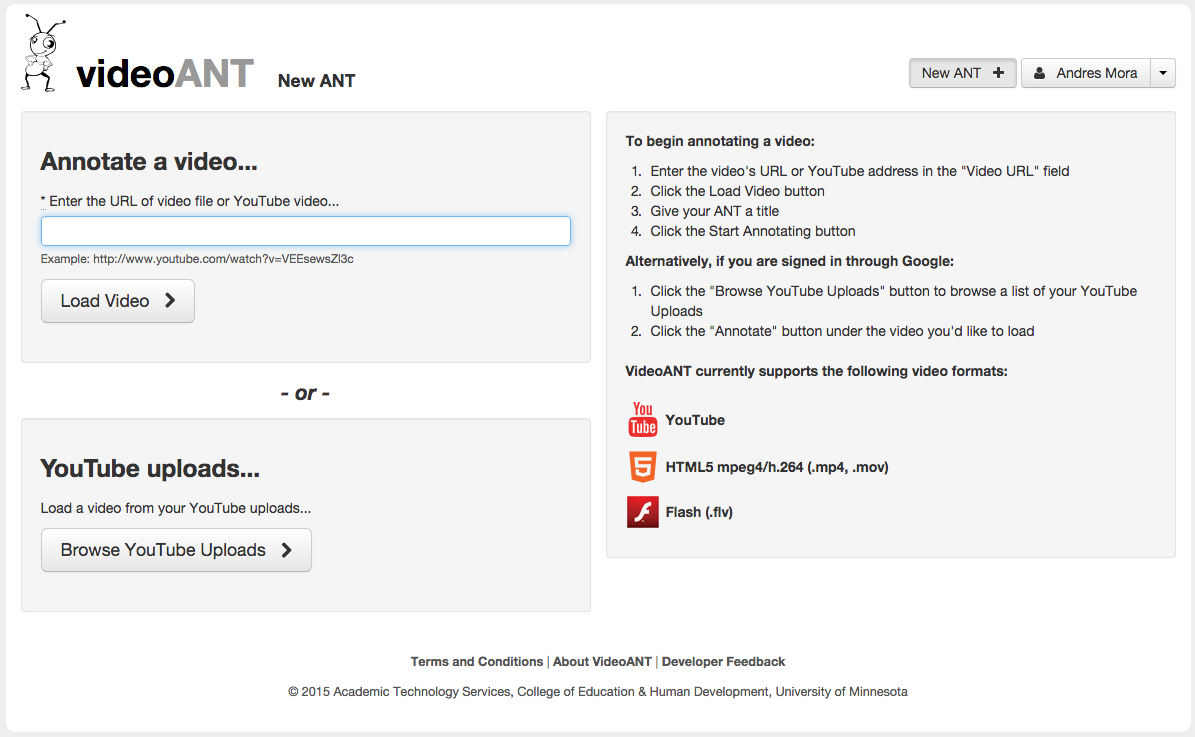
\includegraphics[width=1\linewidth]{images/ant1}
	\caption{GUI de videoANT para la selección de videos.} \label{fig:ant1}
\end{figure}

La Figura \ref{fig:ant2} muestra la GUI de videoANT para el proceso de etiquetado para realizar la segmentación temporal y semántica. En la parte superior cuenta con una barra de progreso del video. En la parte inferior el botón para agregar anotación y luego se procede a brindar unos datos para cada etiqueta, y al final se observa a la derecha como queda cada una de las anotaciones realizadas. Es importante destacar que esta aplicación web únicamente puede realizar las anotaciones con precisión de segundos, y para los objetivos de este proyecto, era necesaria una precisión al nivel de cuadros por segundo. Por ejemplo, un video que tiene una tasa de 30 FPS, se tiene treinta cuadros distintos por segundo y es necesario saber en cual cuadro exacto se da un corte, por lo que solo poder agregar etiquetas en segundos específicos no tiene la precisión necesaria.

\begin{figure}
	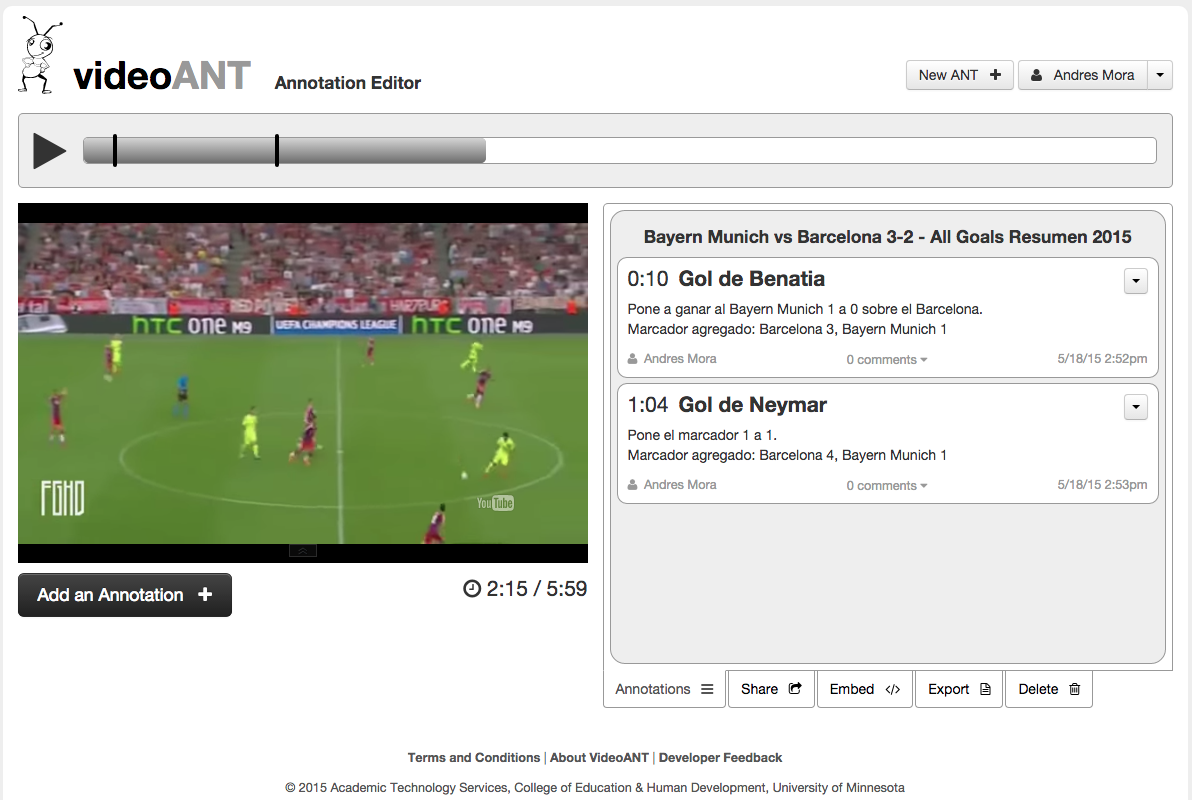
\includegraphics[width=1\linewidth]{images/ant2}
	\caption{GUI de videoANT para realizar la segmentación temporal y semántica.} \label{fig:ant2}
\end{figure}

\subsection{Herramientas realizadas previamente}

\subsubsection{ASPOGAMO}

\subsubsection{ACE}


Del análisis de estas herramientas se puede concluir que ninguna tiene todas las funcionalidades necesarias de forma integral, ni son fáciles de utilizar, por lo que crear una herramienta especializada en la generación de datos de validación es necesario.

\section{\textit{Front-end} y \textit{Back-end}}

\subsection{\textit{Front-end}}

\subsection{\textit{Back-end}}

\section{Frameworks, librerias de software libre para la creación de aplicaciones web}

En esta sección se presentan tres apartados principales los cuales describen las herramientas disponibles en el lenguaje de programación Python, las disponibles en JavaScript y finalmente MongoDB y SQL, dos esquemas de bases de datos diferentes que puede ser utilizados en el desarrollo de aplicaciones.

Un \textit{framework} es una abstracción en la cual un software provee funcionalidades básicas y genéricas las cuales pueden ser utilizadas o modificadas por el programador para crear funcionalidades más específicas para el proyecto que está realizando. En el caso de los \textit{frameworks} para aplicaciones web, estos permiten al programador reutilizar código para manipular \textit{cookies}, acceder a bases de datos, control del ingreso de usuarios, entre otros. Gracias a los desarrolladores de \textit{frameworks}, la programación web ha evolucionado enormemente, ya que estos brindan herramientas que les permite a los programadores concentrarse en el desarrollo de la funcionalidad de su aplicación y no perder tiempo en el caso común de todas las aplicaciones, lo que favorece al prototipado rápido de ideas.

\subsection{Disponibilidad en Python}

Para este lenguaje se estudiaron dos \textit{frameworks} para desarrollo web, Django y Tornado. Los dos son muy utilizados en industria para prototipado rápido, y muchas veces se continúa utilizando en la aplicación final debido a que ambos presentan un desempeño bastante bueno.

\subsubsection{Django}

Django es el \textit{framework} más popular para desarrollo web en el lenguaje de programación Python. Cuenta con diversas funcionalidades como los son la autenticación de usuarios, administración de contenido, mapas del sitio, soporte para RSS. Además cuenta con un \textit{framework} especial para realizar una correcta asignación de memoria caché en el servidor para el acceso eficiente a información recientemente solicitada. [The Django Book, \citet*{django}]

En el tema de seguridad es un \textit{framework} muy completo. Incluye defensas para XSS, CSRF, inyección SQL, Clickjacking, y además cuenta con lo necesario para implementar los sitios HTTP y redirigirlos a su url adecuado en HTTPS. 

Entre las ventajas que tiene se encuentra la popularidad de la herramienta, ya que gracias a esto existe gran cantidad de documentación que puede ser consultada en cualquier momento que se presente una duda con su funcionamiento. De igual manera es común encontrar respuestas a preguntas frecuentes en foros u otros medios.

\subsubsection{Tornado}

Al igual que Django, Tornado es un \textit{framework} muy completo. La mayor diferencia entre ellos es por la razón en la que éste fue creado. Tornado ataca y resuelve en gran medida el C10k, que es uno de los problemas más fuertes que han tenido los servidores en la última década. 

La mayoría de \textit{frameworks} web, como Django, esperan que cada petición realizada sea manejada y procesada por un hilo diferente del servidor. Al tener miles de conexiones simultaneas esta situación hace que el servidor requiera cantidades enormes de memoria para poder manipularlas eficientemente, esto provoca que el servicio se vuelva muy lento o hasta algún fallo más grande que lo obligue a salir de operación.

Para resolverlo, Tornado, a diferencia de Django, y en manera muy similar a nginx y NodeJS, tiene su propio servidor que resuelve las peticiones asincrónicamente, utilizando eventos, asignando poca memoria y de manera predictiva dependiendo de la carga, lo que tiene la enorme ventaja de ser escalable, y de poder manipular muchas conexiones concurrentes manteniendo las necesidades de memoria estables. [Introduction to Tornado, \citet*{tornado}]

Finalmente, Tornado también provee al programador con diferentes funciones genéricas que facilitan la autenticación de usuarios, el manejo de sesiones y cuenta con la biblioteca Motor, que ayuda enormemente a realizar los accesos a bases de datos en la misma manera asíncrona que requiere el servidor.

Esta arquitectura asíncrona es una ventaja para la aplicación que se desarrolla en este proyecto, ya que debe poder manipular gran cantidad de accesos simultáneos de diferentes usuarios, así que Tornado cuenta con esta ventaja por encima de Django. En su contra tiene el hecho de que el modelo de programación por views, y como se realizan los accesos a la base de datos es muy diferente a lo tradicional por ello no es un \textit{framework} que sea para principiantes. Sin embargo, cuenta con bastante documentación oficial para desarrolladores que ven el modelo por primera vez, lo que facilita la labor.

\subsection{Disponibilidad en JavaScript}

En esta subsección se realiza el estudio de algunos \textit{frameworks} disponibles en el lenguaje de programación JavaScript. Este lenguaje ha sido ampliamente utilizado para el desarrollo de \textit{front-end} más interactivos y ha favorecido a que los sitios web no sean solo de contenido estático, sino que permite agregarlo de manera dinámica dependiendo del usuario y además permitió agregar funcionalidades y crear  lo que inició el auge de las aplicaciones web, que en empiezan a competir con algunos softwares locales (que se instalan en la máquina cliente), ya que ofrecen funcionalidades similares, multiplataforma y se pueden acceder prácticamente desde cualquier dispositivo que cuente con un navegador. Los \textit{frameworks} analizados para este trabajo fueron AngularJS, NodeJS y Loopback.

\subsubsection{AngularJS}

AngularJS es un \textit{framework} estructurado desarrollado por Google y utilizado para crear páginas web dinámicas. Con Angular se puede utilizar HTML como lenguaje de etiquetas para generar plantillas de los elementos DOM de un documento web y se utilizan ciertos métodos, que en el \textit{framework} de Angular son llamados directivas, que permiten repetir, mostrar, esconder, animar y manipular el código HTML dándo una impresión más dinámica a la que comúnmente se conoce. [AngularJS Documentation, \cite{angularjsdocs}]

Este aspecto dinámico de la página web se consigue a partir de la combinación del API proporcionado por el \textit{framework} y por medio de diversos scripts personalizados escritos en JavaScript que desarrolle el programador.

Las funcionalidades que proporciona la herramienta se encuentran divididas en 5 tipos principales:

\begin{enumerate}
	\item \emph{funciones}, son métodos como los que se utilizan en cualquier lenguaje de programación. Reciben ciertos parámetros y devuelven un resultado. Es similar al funcionamiento de una biblioteca. Cuenta con métodos como forEach, isArray, toJson, que aunque no proveen una funcionalidad compleja es muy útil tenerlos a mano por ser genéricos.
	\item \emph{directivas}, son el núcleo de Angular. Son las que le dan al HTML las características dinámicas. Algunos ejemplos de ellas son:
	\begin{itemize}
		
		\item ngChange: utilizando los eventos que agrega Angular a los elementos DOM, puede determinar si su valor ha cambiado y así llamar a cualquier método especificado por el usuario. 
		\item ngHide: dependiendo de alguna variable especificada en el código, muestra o esconde ciertos elementos del HTML.
		\item ngKeydown: utilizando eventos, identifica el tiempo que una tecla está siendo presionada, y puede llamar a cualquier función especificada por el usuario en dicho caso.
		\item ngRepeat: a partir de un arreglo de objetos, Angular repite el código HTML contenido en la plantilla cambiando los valores especificados dentro de cada objeto. De esta manera es muy fácil crear listas interactivas, o mostrar información al usuario de manera dinámica.

	\end{itemize}
	
	Para el listado completo de directivas se puede visitar la documentación del API de Angular. [AngularJS Documentation, \cite{angularjsdocs}]
	
	\item \emph{proveedores}, son bibliotecas que proveen información a los diversos servicios a los que se puede acceder en el \textit{framework}. Entre ellos se pueden mencionar el locationProvider y el httpProvider.
	
	\item \emph{servicios}, son diferentes métodos que Angular trae predeterminados o que también pueden ser definidos por el usuario. Estos métodos suelen utilizar información dada por los proveedores para operar. Por ejemplo, el servicio de http permite hacer peticiones del tipo POST, GET, PUT a un servidor. 
	 
	\item \emph{filtros}, es una pequeña sintáxis muy similar al pipeline de Unix que permite dar formato a ciertas cadenas de caracteres para que sean desplegadas de cierta forma. Por ejemplo al realizar \{\{ 2 | currency \}\} lo que se despliega en la página web es \$2.00. Los corchetes dobles ( \{\{\}\} ) son la forma de Angular de saber que eso es proveniente del \textit{framework}, así pueden ser desplegadas variables y se puede aplicar estos filtros.
\end{enumerate}

Angular es una herramienta muy versátil que permite agregar a una aplicación web una cantidad enorme de funcionalidades, por esta razón es uno de los \textit{frameworks} para \textit{front-ends} más utilizados en la actualidad.

\subsubsection{NodeJS}

Al igual que Angular, NodeJS es un \textit{framework} en el lenguaje de programación JavaScript para desarrollo web. Sin embargo, Node no provee las funcionalidades dinámicas para \textit{front-end} de una manera tan fácil e integrada en el HTML como lo hace Angular pero si tiene muchísimas funcionalidades que no solo le permiten ser \textit{front-end} sino también implementar un buen \textit{back-end}.

Trabajando como servidor de \textit{backend}, Node es similar a Tornado en Python. Es asíncrono y lo controlan diferentes tipos de eventos, lo que da los mismos beneficios de escalabilidad y no tiene problemas con manipular muchas peticiones concurrentes ya que realiza eficientes asignaciones de memoria. Además de esta arquitectura que permite tener gran flujo de datos en un solo hilo, en NodeJS también se pueden crear diferentes hijo con el API: child\_process.fork(), permitiendo sacar provecho del paralelismo y de múltiples núcleos del procesador. Utilizando los mismos módulos se puede compartir sockets entre procesos para balancear cargas entre procesadores. [NodeJS Documentation, \cite{nodejsdocs}]

\subsubsection{LoopBack}

LoopBack es un \textit{framework} basado en NodeJS que permite la creación rápida de APIs y la interconexión con diferentes servicios de bases de datos. Es desarrollado y soportado por la empresa StrongLoops [Loopback Documentation, \cite{loopbackdocs}]. LoopBack provee una serie de herramientas que favorecen el desarrollo web ya que está hecho específicamente para la creación de REST APIs.

Entre las mejores características de este \textit{framework} se encuentra el poder definir modelos (que viene a ser la arquitectura de las colecciones o tablas de la base de datos dependiendo de si es un modelo Mongo o SQL, respectivamente) y que el \textit{framework} se encargue de crear ciertos métodos genéricos que por medio de peticiones HTTP como POST, y PUT añada nuevo o modifique el contenido en la base de datos. Estos modelos se definen a partir de ficheros de tipo JSON que funcionan como archivos de configuración para LoopBack. Los JSON se definen con cierta estructura, diciendo si cada uno de los campos es requerido o no para agregar el contenido a la base de datos, y si está o no relacionado a otra colección o tabla. Una vez agregados dichos archivos, se inicia el servicio del servidor de LoopBack y se cuenta con un \textit{back-end} de conexión a la base de datos mínimo pero funcional.

Sumado a estos métodos genéricos, el desarrollador puede añadir diferentes funcionalidades al API por medio del lenguaje de programación JavaScript, de la misma forma en que lo haría si está trabajando en Node, pero no se preocupa por definir el enrutamiento del servidor, solo se dice el URL en el que quiere que esté el servicio y LoopBack se encarga del resto.

Gracias a esta potente funcionalidad, y a que también cuenta con la posibilidad de usar geolocalización, subir y bajar archivos, y notificaciones push para dispositivos móviles, LoopBack es bastante utilizado en la industria. Páginas web como GoDaddy, el Departamento de Energía de los Estados Unidos, y Symantec lo utilizan para administrar comunicarse con sus bases de datos.

\section{Modelos de bases de datos para aplicaciones web}

En esta sección se expone una comparación entre las bases de datos SQL y las NoSQL. Esto con el objetivo de poder decidir, según el tipo de aplicación que se quiere desarrollar, cual de los dos tipos de base de datos que se adapta mejor. Las Tablas \ref{basesDeDatos1} y \ref{basesDeDatos2} muestran una síntesis de la información recopilada.

\begin{table}[H]\centering
	
	\ra{2}
	\caption{Comparación entre los modelos de bases de datos (Parte I)}
	\label{basesDeDatos1}
	
	\begin{tabular}{@{}cC{3cm}C{5cm}C{5cm}c@{}}\toprule
		
		& Característica & SQL & NoSQL &\\ \midrule
		
		& Tipos & Solamente del tipo relacional mediante el lenguaje declarativo SQL. Existen pequeñas variaciones pero se basan en lo mismo. & Muchos tipos distintos. Key-value pairs, basado en documentos, grafos, entre otros &\\ \hline
		
		& Desarrollo & Desarrollado en 1970 para lidiar con la primera ola de aplicaciones con almacenamiento grande de datos & Desarrollados a partir del año 2000 para lidiar con el problema de SQL, esencialmente escalabilidad y datos no estructurados. &\\ \hline
		
		& Ejemplos & MySQL, Postgres, Oracle Database & MongoDB, Cassandra, HBase, Neo4j &\\ \hline
		
		& Modelo de almacenamiento de datos &  Cada archivo nuevo es guardado como una fila en una tabla, y cada columna tiene una porción de información específica para ese archivo, parecido a una hoja de cálculos. Datos de elementos distintos se almacenan en tablas diferentes, y se unen cuando se realiza una búsqueda específica. Por ejemplo si se tiene dos tablas, ``oficinas'' y ``empleados'' y se quiere conocer los números de teléfono de los empleados de una oficina, se asocian las tablas  para adquirir la información completa & Varía dependiendo del tipo de base de datos. For example, key-value stores function similarly to SQL databases, but have only two columns (``key'' and ``value''), with more complex information sometimes stored within the "value" columns. Document databases do away with the table-and-row model altogether, storing all relevant data together in single "document" in JSON, XML, or another format, which can nest values hierarchically. & \\ 
		
		\bottomrule
		
	\end{tabular}
	
\end{table}



\begin{table}[H]\centering
	
	\ra{2}
	\caption{Comparación entre los modelos de bases de datos (Parte II)}
	\label{basesDeDatos2}
	
	\begin{tabular}{@{}cC{3cm}C{5cm}C{5cm}c@{}}\toprule
		
	& Característica & SQL & NoSQL &\\ \midrule
	
	& Esquemas & La estructura y el tipo de datos está definido. Para poder añadir información nueva a algún item, se tiene que alterar toda la base de datos, tiempo durante el cual la base de datos debe salir de operación. & Generalmente son dinámicos. Se puede añadir cualquier información de inmediato, no existe la limitación de tener que cambiar toda la estructura de la base de datos. &\\ \hline
	
	& Escalabilidad & Vertical. Un solo servidor debe ser más poderoso para mayor demanda. Se puede expandir SQL sobre varios servidores, pero se debe de realizar una ingeniería mayor. & Horizontal. Para aumentar la capacidad, el administrador puede añadir más servidores o instancias en la nube, y la base de datos se expande entre los servidores automáticamente de ser necesario.&\\ \hline
	
	& Modelo de desarrollo & Combinación de open-source (SQL) con software propietario (Oracle) & Open-source &\\ \hline
	
	& Soporte de transacciones & Si, se pueden configurar para que los cambios sean totales o que no se realicen del todo. & Son soportados dependiendo de las circunstancias y el nivel. Por ejemplo transacciones a nivel de documentos o nivel de base de datos. &\\ \hline
	
	& Manipulación de datos & Es un lenguaje específico utilizando Select, Insert, Update, entre otros. Por ejemplo: SELECT fields FROM table WHERE… & Se hace a través de APIs orientadas a objetos &\\ \hline
	
	& Consistencia & Se puede configurar para tener alta consistencia & Depende de cual base NoSQL. MongoDB provee alta consistencia, mientras que Cassandra por ejemplo, provee consistencia eventual. &\\ 
	
	\bottomrule
	
\end{tabular}

\end{table}

\clearpage


\section{Patrón de diseño MVC}

El Model View Controllor es un patrón de arquitectura de software que permite hacer una separación entre la interfaz de usuario, los datos, y un módulo encargado de gestionar los distintos eventos y realizar la comunicación entre los dos primeros. El esquema tradicional de MVC se puede observar en la Figura \ref{fig:mvc}.\\

En dicho patrón de diseño, los módulos encargados de la interacción directa con el usuario pertenecen al tipo View. En él se incluyen funcionalidades como desplegar información al usuario o aceptar sus acciones como entradas al sistema. Esta información es enviada el Controller, el cual toma dos tipos diferentes de acción dependiendo de la entrada recibida: acción que \textbf{no altera} el contenido de los datos, pero si afecta la manera en la cual los datos se están visualizando; o la acción que \textbf{si altera} el contenido de datos. Por ejemplo se puede tener la acción de hacer scroll en un documento la cual simplemente afecta la visualización, o la acción de escribir o borrar en el documento que si afecta el contenido de los datos. En el primero de los casos, el encarado de actualizar el View es el Controller, en el segundo caso, es el Model, luego de que el Controller tome las medidas necesarias para variar los datos. Esto se realiza de esta manera para que la sincronización de tareas sea correcta. Finalmente existe un tipo de operación más, y es cuando el View realiza una solicitud al Model para conocer el estado actual de la aplicación, y el Model actualiza de una vez el View. En este tipo de interacción, la solicitud y resultado son triviales, por lo que no se requiere intervención del Controller para realizar la comunicación.\\

\begin{figure}
	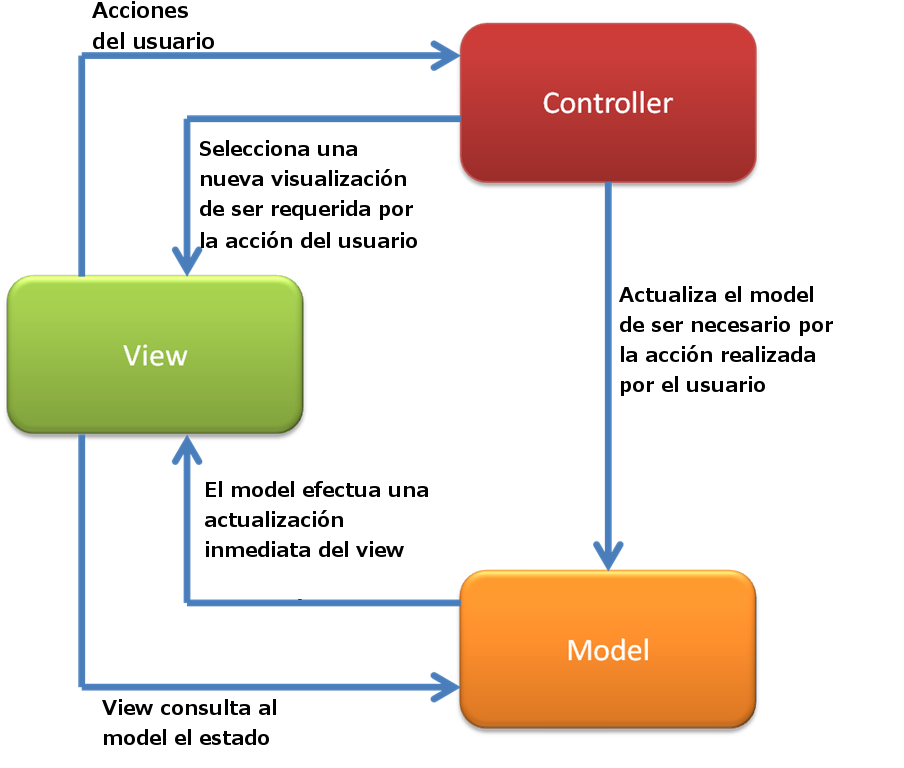
\includegraphics[width=1\linewidth]{images/mvcbase}
	\caption{Patrón de diseño MVC} \label{fig:mvc}
\end{figure}


Existen variaciones de este patrón de diseño, como por ejemplo la versión de MVC implementada por Cocoa, el sistema de interfaces de usuario implementado por los dispositivos de Apple, tanto en los sistemas operativos iOS u OS X. En esta versión alternativa, se limita por completo la interacción entre el View  y el Model, las consultas de estado se deben realizar también por medio del Controller, la información viaja de nuevo a través del Controller, y finalmente este es el encargado de actualizar el View de manera acorde.
